\documentclass[11pt, a4paper, twoside]{article}

%% Die folgende Anleitung gilt für Linux:
%%
%%  Die Übersetzung dieses Dokuments erfolgt mit (ggf. öfter aufrufen):
%%  pdflatex seminar.tex
%%
%%  Falls die Bibliographie geändert wurde, dann zusätzlich:
%%  bibtex seminar
%%
%%  Bitte darauf achten, dass pdflatex und bibtex keine Warnungen und
%%  keine Fehler melden.
%%
%%  Das Ergebnis kann man ansehen:
%%  acroread seminar.pdf
%%
%%  Die Quelldatei einer deutschen Rechtschreibprüfung unterziehen:
%%  ispell -d deutsch -T latin1 seminar.tex

%% Kodierung des Dokuments
\usepackage[utf8]{inputenc}

%% Titel und Autor der Ausarbeitung (BITTE ANPASSEN!)
\title{The Memento Design Pattern}
\author{Daniel Geier}
\date{} %% leer lassen

%% Grafiken einbetten
\usepackage{graphicx}

%% Verweise in der PDF
\usepackage{hyperref} % important: load after float
\hypersetup{
	pdfproducer={pdfeTex 3.14159-1.30.6-2.2},
	colorlinks=false,
	pdfborder=0 0 0	% keine Box um die Links!
}
\usepackage{url}
\urlstyle{rm}

%% Programmcode Listings
\usepackage{listings}
\lstset{basicstyle=\ttfamily}

\lstset{language=C++,
	basicstyle=\ttfamily,
	keywordstyle=\color{blue}\ttfamily,
	stringstyle=\color{red}\ttfamily,
	commentstyle=\color{green}\ttfamily,
	morecomment=[l][\color{magenta}]{\#},
	frame=single,
	numbers=left
}

\usepackage{color}
\usepackage{framed}

%% Seitenlayout (BITTE NICHT VERÄNDERN!)
\oddsidemargin0mm
\evensidemargin0mm
\textwidth159.2mm
\topmargin0mm
\headheight0mm
\textheight43\baselineskip

%% Header und Footer (BITTE NICHT VERÄNDERN!)
\usepackage{fancyhdr}
\pagestyle{fancy}
\fancypagestyle{plain}{\fancyhf{}\fancyfoot[RO,LE]{\thepage}\renewcommand\headrulewidth{0pt}}
\fancyhf{}
\fancyhead[LE]{\myauthor}
\fancyhead[RO]{\mytitle}
\fancyfoot[RO,LE]{\thepage}
\setlength{\headheight}{14pt}
\makeatletter
\let\mytitle\@title
\let\myauthor\@author
\makeatother

\def\cpp{C{}\texttt{++}}

% Der eigentliche Inhalt startet hier
\begin{document}
	\maketitle
	
	% GitHub notice
	\begin{framed}
		\noindent\textcolor{red}{Hinweis: Die aktuellste Version gibt es immer auf GitHub. Ihr seid herzlich dazu eingeladen, Issues aufzumachen!\footnotemark}
	\end{framed}
	\footnotetext{\url{https://github.com/danielgeier/The-Memento-Design-Pattern/blob/master/the_memento_pattern.pdf}, \url{https://github.com/danielgeier/The-Memento-Design-Pattern/issues/new}}

	\begin{abstract} \noindent
 		Managing state restoration is a commonly occurring task in software development. Memento is a design pattern used for saving and restoring the (partial) state of objects. After examining reasons for using Memento, a comprehensive overview covering the static and dynamic structure is given. Examples from a \cpp{} source are presented. Benefits, drawbacks and implementation details in \cpp{} and \verb|Java| are discussed.
	\end{abstract}
	
	\section{Introduction}
	\label{sec:intro}
	The average project size in software development is constantly growing and so is code complexity. On the technical side, design patterns, made popular by Gamma \textit{et al.} \cite{gamma1993design}, are an attempt to tame this complexity with a structured object-oriented approach. The impact of design patterns were critically examined in a number of empirical investigations (e.g., \cite{bieman2003design}, \cite{porras2010empirical}, \cite{jeanmart2009impact}, \cite{khomh2008design}, \cite{di2008empirical}, \cite{prechelt2001controlled}, \cite{vokac2004defect}, \cite{vokavc2004controlled}), which led to mixed conclusions on the benefits patterns may bring. Nonetheless patterns, when carefully used, can bring key advantages to the design and implementation process.
	
	The analysis in this paper concentrates on the Memento design pattern as it is presented in \cite{gamma1994design}.
	
	\section{Motivation}
	\label{sec:motivation}
	 When preserving the state of an object, the first technique that comes to mind is copying the variables that represent the state and copy them back to the object at a later time. Though seductive in its simplicity, this technique breaks encapsulation. Another possible solution, letting the stateful object manage its previous states by itself, violates separation of concern.\footnote{Section~\ref{sec:benefits} has more details on the benefits of encapsulation and the separation of concerns.}
	 
	 Memento works by splitting the burden of managing state restoration between multiple classes, thus observing good development practices.
	 	
	\section{Structure}
	\verb|Originator| is the class whose state will be encapsulated by our memento.
	
	\verb|Caretaker| is the user of the originator. It is responsible for storing the mementos returned by the originator and returning them back to it. The caretaker never accesses the memento directly.
	
	\verb|Memento| encapsulates the state of the originator. It provides set and get mechanisms for this state which is accessible only by the originator. This is achieved by defining a \emph{narrow} interface for the caretaker and a \emph{wide} one for the originator.
	
	\begin{figure}[htb]
		\begin{center}
			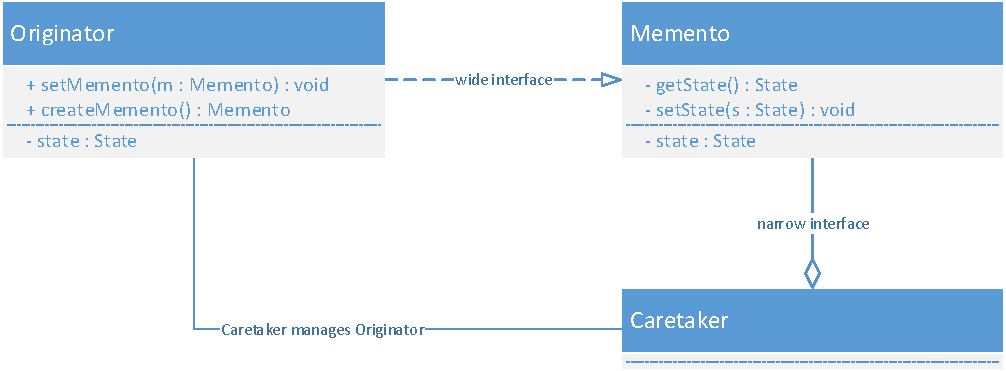
\includegraphics[width=\textwidth]{class_diagram.pdf}
			\caption{Class diagram showing the static structure with classes, their methods and class variables used}
			\label{fig:class}
		\end{center}
	\end{figure}
	
	As one can see in figure \ref{fig:class}, \verb|Originator| implements the method \verb|createMemento| for creating a memento, while \verb|setMemento| is used to load the previous state. \verb|Memento| implements accessors for its state, which should only be accessible to the \verb|Originator|. \verb|Caretaker| doesn't implement any methods specific to the pattern.
	
	The key to Memento lies in implementing two different interfaces for \verb|Originator| and \verb|Caretaker|. The details of \verb|Memento| should be opaque to all but \verb|Originator| which accesses \verb|Memento| through a \emph{wide} interface. All other participants interact with \verb|Memento| through an \emph{narrow} interface, which leaves \verb|Memento| opaque to them. This poses difficulties in programming languages who lack mechanism to define such constructs. Section~\ref{sec:impl} discusses mechanisms in \cpp{} and \verb|Java| for defining those interfaces.
	
	\begin{figure}[htb]
		\begin{center}
			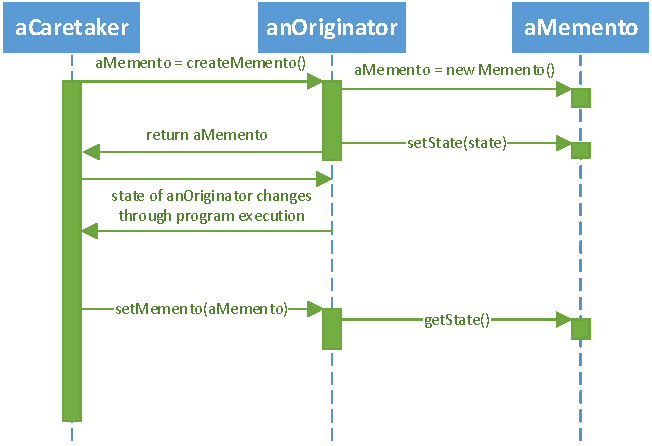
\includegraphics[width=0.9\textwidth]{sequence_diagram.pdf}
			\caption{Sequence diagram showing the dynamic structure through method calls being made}
			\label{fig:sequence}
		\end{center}
	\end{figure}
	
	Figure \ref{fig:sequence} shows how the pattern is used in practice. \verb|aCaretaker| receives \verb|aMemento| from \verb|anOriginator| and saves it through the subsequent program execution. As soon as \verb|aCaretaker| wants to restore \verb|anOriginator| to a previous state, it returns \verb|aMemento| back to \verb|anOriginator| through the \verb|setMemento| method.
	
	
	\section{Sample Code}
	The sample application is a Mandelbrot\footnote{Observations about the intrinsics involved in the calculation of the Mandelbrot and related fractals are made in \cite{mandelbrot1980fractal}.} fractal explorer written in \cpp. The fractal drawing and rendering is managed in the \verb|Mandelbrot| class. It is responsible for calculating the values of the Mandelbrot set and saving them in a array of pixels.
	
	\begin{lstlisting}[language=c++, caption={Mandelbrot.h}]
	class Mandelbrot
	{
	public:
		Memento* createMemento();
		void setMemento(Memento* memento);
		
		/* ... */
		
	private:
		friend class Memento;
		
		// Variables saved within the memento
		Dimensions bounds;
		uint32_t* pixels;
		
		// Independent state variables
		int iterations;
		int width, height;
		bool doCalc;
		
		/* ... */
	};
	\end{lstlisting}
	
	The Memento pattern is used for saving the state of the calculation and the calculated image.
	
	\begin{lstlisting}[language=c++, caption={Mandelbrot.cpp}]
	Memento* Mandelbrot::createMemento()
	{
		Memento* m = new Memento();
		m->setPixels(pixels, width * height);
		m->setBounds(bounds);
		return m;
	}
	
	void Mandelbrot::setMemento(Memento* memento)
	{
		memcpy(pixels,memento->getPixels(),
			width * height * sizeof(uint32_t));
		bounds = memento->getBounds();
		doCalc = false;
	}
	\end{lstlisting}
	
	The \verb|Memento| class saves the state which consists of the image data, \verb|pixels|, and the logical position of the Mandelbrot section, \verb|bounds|.
	
	A wide interface to \verb|Mandelbrot| is achieved by declaring it a \verb|friend| (see Section~\ref{sec:impl}).
	
	\begin{lstlisting}[language=c++, caption={Memento.h}]
	class Memento
	{
	public:
		~Memento();
		
	private:
		friend class Mandelbrot;
		
		uint32_t* pixels;
		Dimensions bounds;
		
		Memento();
		void setPixels(uint32_t* oldPixels, int size);
		void setBounds(Dimensions bounds);
		
		uint32_t* getPixels();
		Dimensions getBounds();
	};
	\end{lstlisting}
	
	\begin{lstlisting}[language=c++, caption={Memento.cpp}]
	void Memento::setPixels(uint32_t* oldPixels, int size)
	{
		pixels = new uint32_t[size];
		memcpy(pixels, oldPixels,
			size * sizeof(uint32_t));
	}
	
	void Memento::setBounds(Dimensions oldBounds)
	{
		bounds = oldBounds;
	}
	
	Memento::~Memento()
	{
		delete[] pixels;
	}
	
	uint32_t* Memento::getPixels()
	{
		return pixels;
	}
	
	Dimensions Memento::getBounds()
	{
		return bounds;
	}
	\end{lstlisting}
	
	In the main event loop, \verb|zoomIn| is called, when the eponymous action is to be performed. A memento is created and put aside in dynamic storage.
	
	\begin{lstlisting}[language=c++, caption={Main.cpp}]
	void zoomIn() {
		mementos.push_back(mandelbrot.createMemento());
		mandelbrot.zoomIn(zoomRect);
		mandelbrot.render(renderer, screenTexture);
	}
	\end{lstlisting}
	
	\verb|zoomOut| is called, when the user wants to return to the previous section of the fractal. A memento is retrieved from storage and the state of the \verb|Mandelbrot| object restored.
	
	\begin{lstlisting}[language=c++, caption={Main.cpp}]
	void zoomOut() {
		if (mementos.size() > 0) {
			Memento* m = mementos.back();
			mementos.pop_back();
			
			mandelbrot.setMemento(m);
			mandelbrot.render(renderer,
				screenTexture);
			
			delete m;
		}
	}
	\end{lstlisting}
	
	\section{Discussion}
	
	\subsection{Benefits}
	\label{sec:benefits}
	\emph{Encapsulation}. Encapsulation has been shown to provide key benefits in the understandability and changeability of a computer program \cite{snyder1986}. As already explored in Section~\ref{sec:motivation}, simply copying member variables is unsuitable for maintaining good development practices; exposing state variables involves confiding implementation-specific details of the class. The memento object encapsulates the state of the originator. Inaccessible for all but the originator, the state is safe from unsound modifications from outside objects. \\
	
	\noindent\emph{Separation of concerns\footnote{An excellent source on separation of concerns is \cite{Huersch95}.}}. Before using Memento, the originator had to manage all state-restoring functionality by itself to maintain proper encapsulation. With this functionality moved into Memento, the originator is simplified.
	
	\subsection{Drawbacks}
	\emph{Memory overhead}. Depending on how easily the state can be refactored out of the originator, there may be a substantial memory overhead in creating a memento. \\
	
	\noindent\emph{Defining different interfaces}. Some programming languages may lack facilities for declaring both a narrow and wide interface. \\
	
	\noindent\emph{Hidden costs}. As the implementation of the memento is hidden from the caretaker, it doesn't know how much state the memento is managing. It will therefore be hard to assess the memory consumption of a possibly otherwise lightweight caretaker.
	
	\subsection{Implementation Details}
	\label{sec:impl}
	In Java, \emph{static nested classes} can access private members of its surrounding class and vice versa. In such a way the memento can be implemented as a static nested class of the originator class.
	
	In C++ the \verb|friend| keyword signals that the stated class may access private members of the class. Hence the memento has to declare the originator as a \verb|friend|, as does the originator with the memento.
	
	\bibliographystyle{plain}
	\bibliography{the_memento_pattern}
\end{document}
